\chapter{Visualisation Evaluation}\label{C:eval}
Following the completion of the implementation stage of this project a final
user evaluation was carried out on the visualisation. This evaluation was
primarily designed to discover whether or not the visualisation created was
successful in fulfilling the requirements of the project.

\section{What did we do}
\section{Why did we do it}
Visualisation methods are often designed and evaluated by presenting 
results informally to potential users. No matter how 
efficient a visualisation technique may be, or well planed it is, if it does
not convey information 
effectively, it is of little use. User studies offer a 
scientifically sound method to measure a visualisations 
performance. There are many reasons to pursue user studies. Studies can 
be used to evaluate the strengths and weaknesses of 
different visualization techniques or show that a visualization technique is 
useful in a practical sense, according to some objective 
criteria, for some specific task \cite{kosara2003thoughts}. 
The fundamental goal of conducting user studies is to 
seek insights into why particular visualisation techniques are effective.
\cite{kosara2003thoughts}.

The evaluation of this project was designed to qualitatively assess users
reactions and experiences with the IKVT. By mapping users experiences to the
project requirements I was able qualitatively evaluate how successful the
visualisation
was a fulfilling these requirements. Qualitative evaluation was chosen over
quantitative because of 3 main reasons ....~

\section{Experimental Design}
\subsection{Expectations of evaluation}
From this evaluation the expectations were that users would take approximately 3
minutes to feel comfortable with using the visualisation for the basic tasks of
moving the camera around, sorting the exoplanets, and using the range sliders to
filter the exoplanets. 

Following this accostomisation time it was expected that users could accurately
complete the set of questions in a worksheet (APPENDIX QUESTIONS) whilst using
the visualisation. During this stage users are expected to use both interaction
methods (Keyboard \& Mouse, and Kinect sensor). During the keyboard \& mouse
portion of the experiment the users should make more accurate selections and
exhibit more effective data seeking behavior, whereas during the Kinect portion
they would be more interesting in experimenting with gestures rather than
attempting to gain information about exoplanets. 

When users have finished using the visualisation and fill in the questionnaire
asking them about their experiences with the system the expectation was that
they would detail the areas of the visualisation that ...~

\subsection{Participants}
The user study was undertaken by 9 participants P2 to P10 as well as a 1 user
pilot study by P1. All were either students or
young professionals from a mix of specialties aged between 21 to 26 with a mix
of genders with 5 females and 4 males. 5 of these participants had extensive
prior experience with Kinect sensors, and all participants had experienced a 3D
visualisation before.

\subsection{Evaluation Environment}
\begin{figure}[H]
  \centering
      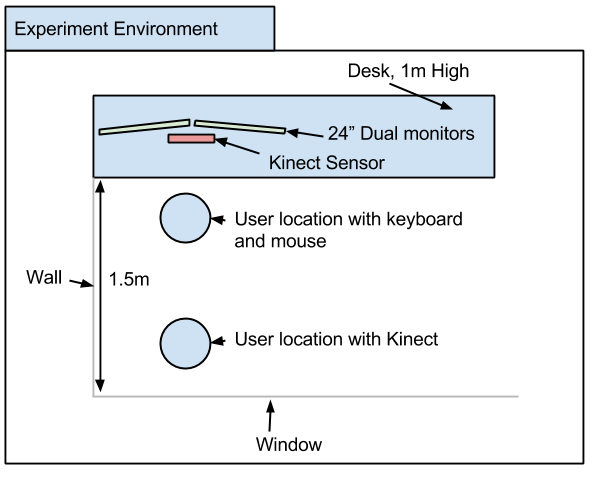
\includegraphics[width=0.8\textwidth]{images/environment.png}
  \caption{Evaluation environment}  
    \label{fig:environment}
\end{figure}


\subsection{Evaluation Method}
A poorly designed experiment will only yield results of limited value, because
of this it was important to ensure that each stage of the experiment was
focused on evaluating a specific area of the visualisation in relation to the
project requirements. There were 3 key methods of gathering results during this
evaluation; a
worksheet to fill out whilst using the visualisation made up of 2 sets of
questions(one for the keyboard \& mouse system and one for the Kinect
system)(APPENDIX), a questionnaire to
fill in afterwards about the experience (APPENDIX), and the examiners
observations about
how the users interacted with the system.  
\\\\
The following are the steps that were carried out during each user evaluation to
ensure that the variables were the same each time
\begin{itemize}
\item The user enters the room and sits down at the computer.
\item They are handed the consent form and information sheet.
\item After these are completed they are handed the user questionnaire and the
set of questions to answer while using the system. On this questionnaire there
are two sets of questions, the first is for the keyboard and mouse system, and
the second if for the Microsoft Kinect system.
\item They are then given a brief introduction into each of the visualisation
components and what the visualisation as a whole represents
\item Following this they are advised that they have 5 minutes to get
familiarised with the system but they do not need to use all of this time (the
amount of time taken will be recorded for analysis of how user friendly and
intuitive the system is).
\item Following this the user is asked to complete the worksheet by first
using the mouse and keyboard system. When they feel they have answered the first
set of questions they will notify the examiner who will move the user to the
Kinect
system to continue with the second set.
\item Once the user has completed both sets of questions they are asked to fill
in the qualitative user questionnaire about their experiences using the
visualisation. 
\item Following this if the examiner has no follow up questions the user is free
to leave.
\end{itemize}

\subsection{Pilot Study}
Due to the significant costs associated with running an experiment, it 
is valuable to conduct a pilot study with one or two 
participants. This allows testing and refining the experimental
design before starting a full-fledged study with numerous 
participants \cite{kosara2003thoughts}. 

The reason for conducting a pilot study for this project was to ensure that
the experiment was
producing the data needed to evaluate the visualisation produced as well
as taking the correct amount of time to complete. In addition to this it was
used to discover whether there were any aspects of the study that would
interfere with the results. One participant was asked to take part in a pilot study before any results were
collected, this participant is referred to as P1. This participant was asked to
complete all of the activities that
make up the main experiment. This pilot study took approximately 15 minutes as
intended, this included the time needed for the explanation and completion of
paperwork, as well as the experiment itself.

P1 successfully each of the questions whilst using the visualisation with only
limited assistance from the examiner. This assistance was required due to the
wording of
some of the tasks users were asked to complete being ambiguous which caused
unnecessary confusion which could have interfered with the results. These
ambiguous questions and
tasks were removed prior to the main user study. During the main study only P4
and P10 asked for clarification on the questions or tasks.

P1 had some initial difficulty using the range sliders but after a small period
of experimentation began using them for the majority of tasks which turned out
to be very efficient. P1 also found that whist the range sliders were effective,
they did not allow fine enough control for making small changes. The component of the visualisation that P1 had the most difficulty was using the
view depicting the location of planets in relation to their stars habitable
zones. This difficulty seemed to stem from the lack of a common point of
reference for each planet due to each planet having a different star with its
own habitable zone.

During the Kinect portion of the experiment P1 found that being in a sitting
position whist interacting with the visualisation did not feel natural due to
``being required to reach out and exert effort to hold an upright position of
the arms for an extended period of time''. The following figure displays P1s
reactions to questions about the experience of using the IKVT.
\begin{figure}[H]
  \centering
      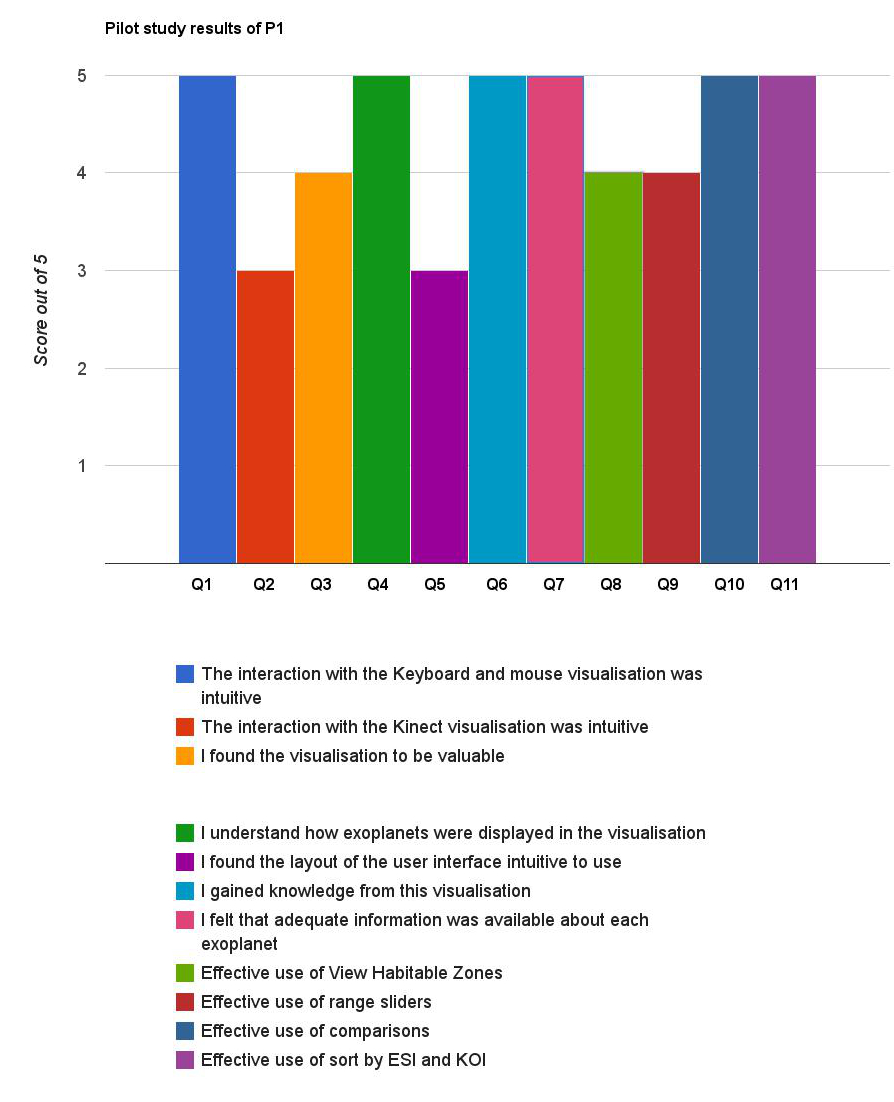
\includegraphics[width=1\textwidth]{images/pilot.jpg}
  \caption{Pilot study results of P1}  
    \label{fig:pilot}
\end{figure}





\section{Results}
The keyboard \& mouse portion of the experiment was primarily intended to
evaluate how the interaction techniques that were introduced into the
visualisation can aid users in their information seeking behaviors.
This was evaluated through the first part of the question set that users filled
in whilst using the visualisation. These questions were designed in a way that
encouraged users to make use of each of the interactive features that were
introduced.

The Microsoft Kinect portion of the experiment was intended to evaluate how
users would react to interacting with the visualisation by gesture. The
questions for this portion of the evaluation were designed to find out users
experiences with interacting via Kinect.

\begin{figure}[H]
  \centering
      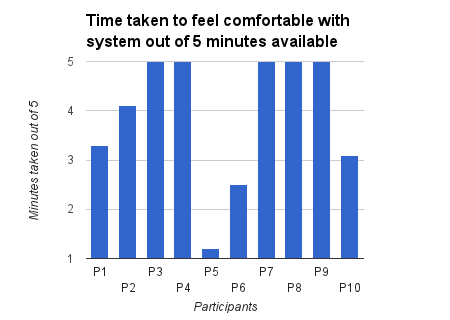
\includegraphics[width=0.8\textwidth]{images/timeTaken.png}
  \caption{Amount of time taken for users to feel comfortable with
visualisation}  
\end{figure}


\begin{enumerate}
 \item[P2.] 
 P2 found that the information displayed in the IKVT was easy to follow even
without knowing exactly what each piece of information actually meant.
 
 P2 also found that without more of an in depth introduction into each of the
tools 
 
 P2 Did not realise that it was possible to move the camera around until it was
performed accidentally.
 
 P2 had trouble when moving between questions on the worksheet due to forgetting
to reset the range sliders after using them.
 
 P2 sometimes got confused after changing the view multiple times which caused a
loss of perspective.
 
  ``Do exoplanets actually exist''
  
  P2 had trouble with Habitability zone

   Spent lots of time playing with the Kinect sensor due to the novelty of it.
   
   Had trouble when zoomed in to far with the Kinect sensor due to getting
flustered
   
   P2 predicted that if there was more time to use the visualisation they would
have felt more comfortable and learned more rather than focusing on trying to
use it.
   
   Found the layout easy to use and simple to understand however found the range
sliders slightly confusing.
   
   Found the outline of the user in the background of the visualisation useful
for maintaining perspective of where they were interacting with the system
   
   Found that all of the information was layed out clearly in the text area.
This information was interesting

   The text size of the interaction panel could have been bigger to make it more
easy to glance at.
   
  \item[P3.]
   \item[P4.]
   P4 found that the key strengths of the system was the ability to sort
exoplanets, zooming.
   
   P4 found that the range sliders were not intuitive. P4 also found that the
zooming out speed was not fast enough in the kinect system. Also found that the
rotation speed was to fast.
   
   P4 suggested improvements of making a more consistent speed of zooming and
making the range sliders more intuitive.
   
   P4 found that the mouse system was more useful for gaining information due to
increased accuracy and because the Kinect was more of a novelty and so more time
was spent preoccupied by playing with it rather than looking at the text area.
   
    Keyboard and mouse were easier due to being used to using them.
    
    The body movements for the kinect were what P4 expected but the speeds at
which the visualisation responded were not as expected
   
   P4 did not have any experience looking at 3D visualisations and had only used
2D graphs.
   
   P4 understood the attributes of the exoplanets bu found it hard to read them
and interpret the visualisation at the same time.
   
   Due to the size of the text in the information panel being size 12font it was
difficult to read quickly. The range tool was also hard to use due to its size. 
   
   P4 also wanted more control over where the camera was centered.
   
    P4 felt that more work needed to be put into making the information stand
out at the user rather than needing to be ``searched'' for.
    
    P4 felt that using IKVT broadened her perception of how information can be
graphically represented.
   
   P4 also felt that the names of some of the attributes were not made clear
enough (Eg, ESI, KOI).
  \\\\
  Notes
  \\
  P4 seemed to have more difficulty using the visualisation than the other
users.
   
    \item[P5.]
    P5 found the kinect was fun and very engaging. He found that the use of size
and colours of the visualisation were useful for making the information easy to
understand
    
    P5 also found the zooming effect that occurred when planets were filtered
with the range sliders useful for making more accurate selections.
    
    P5 found that some of the strengths of the visualisations were that is gave
a sense of the space between exoplanets, the size and the vast numbers of them.
    
    P5 found that because the information panel was not central in the
visualisation that it required effort to break away from the main visualisation
window which broke the immersion.
    
    P5 felt that limiting the amount that the user could move around in the
visualisation(stop being able to go to unnecessary places) would be an
improvement, especially in the graph view.
    
    P5 found that the mouse \& keyboard system was the most effective for
gaining information due to the accuracy that it afforded the user and the fact
that it required less time to learn the gesture based controls and more time
exploring the data.
    
    Kinect required more of an introduction than was given
    
    P5 found that having the visuals interactive and organised made it better to
understand the complex information.
    
    P5 felt that the layout of the interactive components were fine but could be
improved by making them ``pop out more''
    
     \item[P6.]
     
     P6 did not initially spot the text areas changing as planets were selected
until reading the worksheet
     
     P6 had difficulty with habitability question.
     
     P6 found that using the Kinect sensor was the most fun and enjoyed the
method of hand recognition.
     
     P6 also liked being able to change between views in the visualisation
     
     P6 found that the interaction panel was ``simple - not filled with to much
information'' and so was easy to use.
     
     She found that the use of 3D components and being able to change views,
move the camera around for better viewing angles, and zooming in and out were
some of the key strengths of the system.
     
     P6 also found that being able to sort the planets according to attributes
and then filtering them to remove the planets she did not want was a powerful
tool.
     
     P6 felt that a weakness of the Kinect sensor was that it detected the whole
hand rather than a more controllable interface like a finger.
     
     However P6 did find that the 3D camera was sometimes difficult to control
     
     A suggestion for the system was that smoother movements of the camera and
planets could be incorporated and refine it to make it more user friendly so
that it can be used without any explanation.
     
     A further improvement would be to make the menu more aesthetically
pleasing.
     
     P6 found the mouse \& keyboard system the easiest to use because it was the
interactive method that she had the most experience with.
     
     P6 found that the interactive method that allowed the most learning was the
mouse \& keyboard. This was because more time was spent with it and because she
was closer to the screen and so could read the textual information better. P6
found that she used more time playing around with the Kinect system trying to
select planets rather than trying to get information.
     
     P6 felt that the seating location was to far away to accurately see what
she was selecting with the Kinect sensor.
     
     P6 noted that a system like this would be perfect for use in schools and
education centers and would interest many people.
     
     P6 felt that a key improvement would be to have used more 2D views over 3D
views and to make the interaction panel and visualisation panel more
aesthetically similar to ``connect them together''.
     
      \item[P7.]
      P7 found that the visualisation was very easy to use and the way that she
was able to control the exoplanets was fun.
      
      P7 found that a weakness of the system was that it displayed to much
information at once which was confusing. 
      
      P7 also found that the keyboard and mouse system was the most useful as it
felt more natural and allowed access to more information as well as making it
easier to access the information she wanted.
      
       \item[P8.]
       P8 liked being able to toggle between the different planetary sorting and
filtering. He also found that the Kinect system was more fun to use but lacked
the control that the keyboard \& mouse allowed.
       
       P8 also found that the visualisation was informative and a ``neat'' way
of visualising what would normally be stacks of information that he would
struggle to navigate.
       
       P8 found that a weakness of the system was that there was a lot of
concepts that needed to be understood about the planets and so a glossary would
have been an improvement. 
       
       He also found that the lack of movement space while using the Kinect made
it harder to use it freely.
       
       He also found that overlapping planets made it hard to make selections
with the Kinect. He also would have liked a way to cancel a selection without
having to select another planet.
       
       P8 found that the keyboard \& mouse system gave more control and access
to the filters and sorting.
       
       P8 found that he learned many things whilst using the visualisation and
gained an interest in learning more about Exoplanets which he previously had no
real interest in.
      
        \item[P9.]
        
        P9 found it very easy to make comparisons between exoplanets due to the
sorting ability.
        
        
        P9 enjoyed the Kinect side of the visualisation due to it allowing her
to get a sense of the scale of exoplanets found.
        
        P9 found that the strengths of the visualisation with regard to the
Kinect system were that it allowed a fun way of interacting with a serious
visualisation. The ability to rotate the system with its realistic 3D as well as
select specific planets and zooming in an out made it very effective.
        
        The keyboard \& mouse side of the visualisation provided an effective
way of accessing the information thanks to the sorting and filtering ability.
        
        Initially P9 was confused as to where the information was displayed
about each selected exoplanet but once she realised it was very easy to use.
        
        P9 found the keyboard \& mouse system more effective but enjoyed the
interaction with the Kinect system more.
        
         \item[P10.]
         P10 found the animations in the visualisation were enjoyable whilst
exploring
         
         He found that it was easy to compare the information for each exoplanet
and to get a sense of the quality of exoplanets.
         
         P10 found that the interaction panel was good but its location was
awkward with the sliders down the left hand side of the screen.
         
         He found that the keyboard was the most effective interaction method
for exploring the data but the novelty of the Kinect sensor was more fun due to
its novelty
         
         P10 felt that the interaction panel felt like it was hidden and that
there was to much information displayed in it.
         
          \item[Observations.]
         All users had trouble with the understanding the habitability zones of
stars due to there being no standard habitability to compare.
         
         All users that had extensive experience with 3D software adopted the
system much faster than those that hadn't and were in general more comfortable.
         
         All users enjoyed the Kinect version more than keyboard \& mouse even
though it was harder to gain information from the visualisation
         
         Once users worked out how to use the range sliders they used them
extensively
      
\end{enumerate}


\section{Performance evaluation}
Entire render cycle takes less than 

\subsection{Evaluation of Requirements}
\subsubsection{Evaluation of Functional Requirements}
\begin{enumerate}

 \item[R1.] The visualisation needs to display planetary information to convey
knowledge to users.

Successful

 \item[R2.] The visualisation needs to allow exoplanets to be compared against
one another.

Successful

 \item[R3.] The planets need to be able to be ordered by their similarity to
earth (ESI) and by their Kepler Object of Interest number (KOI).
 
Successful
 
 \item[R4.] The visualisation needs to allow users to define ranges of planetary
attributes to filter which planets are displayed.

Successful

 \item[R5.] Users need to be able to view the habitable zones of stars in
relation to the planets orbiting them.

Successful but due to unintuitiveness the usability is reduced

\end{enumerate}

\subsubsection{Evaluation of Nonfunctional Requirements}
\begin{enumerate}
 \item[R6.] All interaction methods must be visible and intuitive.

 Successful but needs to be more prominent
 
 \item[R7.] The visualisation must remain uncluttered to reduce information
overload.

Successful

 \item[R8.]  There needs to be two modes of interaction with the system,
keyboard and mouse vs gesture based.

Successful but Kinect was worse for information seeking.

\end{enumerate}

\begin{figure}[H]
  \centering
      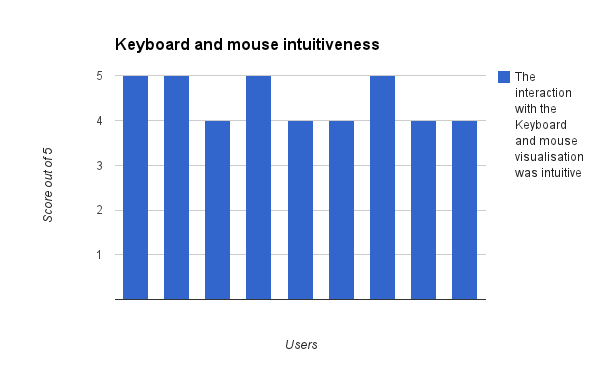
\includegraphics[width=0.8\textwidth]{images/charts/chart_1.png}
  \caption{Intuitivity of keyboard and mouse}  
    \label{fig:chart1}
      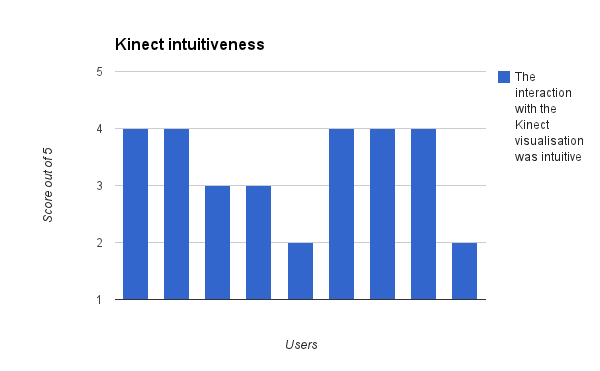
\includegraphics[width=0.8\textwidth]{images/charts/chart_2.png}
  \caption{Intuitivity Microsoft Kinect sensor}  
    \label{fig:chart2}
      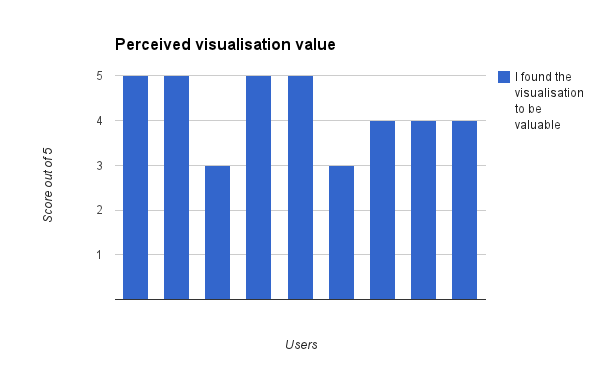
\includegraphics[width=0.8\textwidth]{images/charts/chart_3.png}
  \caption{Perceived value of visualisation}  
    \label{fig:chart3}
\end{figure}

\begin{figure}[H]
  \centering
      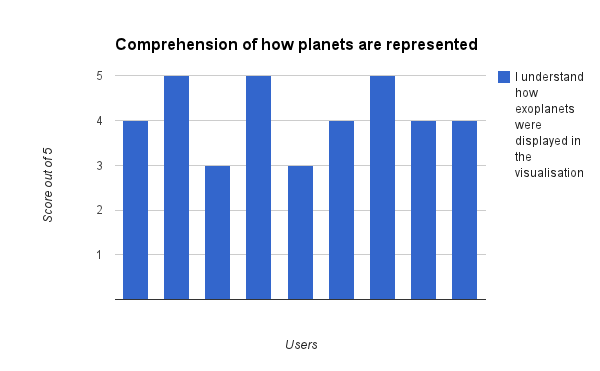
\includegraphics[width=0.8\textwidth]{images/charts/chart_4.png}
  \caption{User comprehension of visualisation}  
    \label{fig:chart4}
      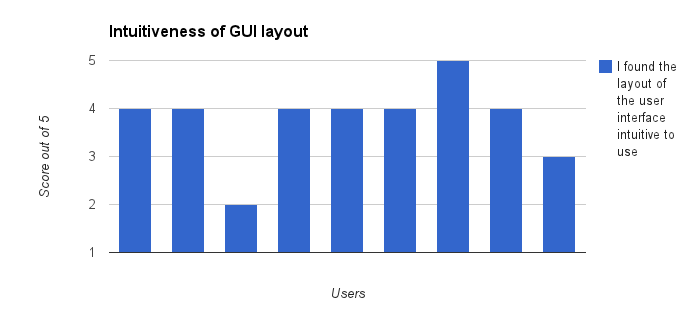
\includegraphics[width=0.8\textwidth]{images/charts/chart_5.png}
  \caption{GUI layout intuitivity}  
    \label{fig:chart5}
\end{figure}

\begin{figure}[H]
  \centering
      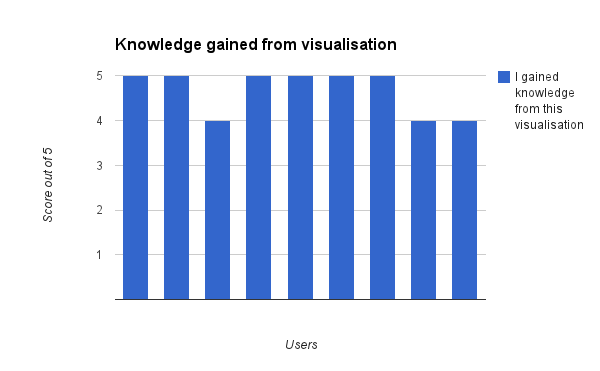
\includegraphics[width=0.8\textwidth]{images/charts/chart_7.png}
  \caption{Knowledge gained from the visualisation}  
    \label{fig:chart7}

      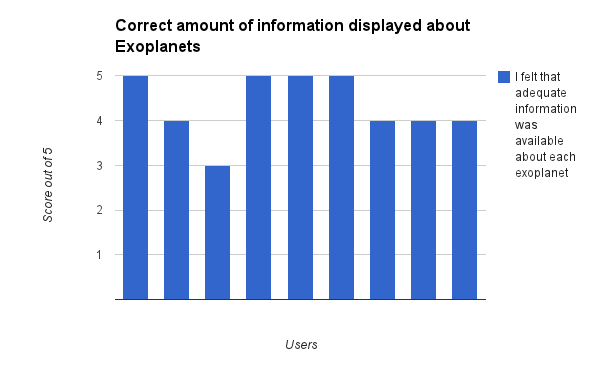
\includegraphics[width=0.8\textwidth]{images/charts/chart_8.png}
  \caption{Correct amount of information displayed}  
    \label{fig:chart8}
      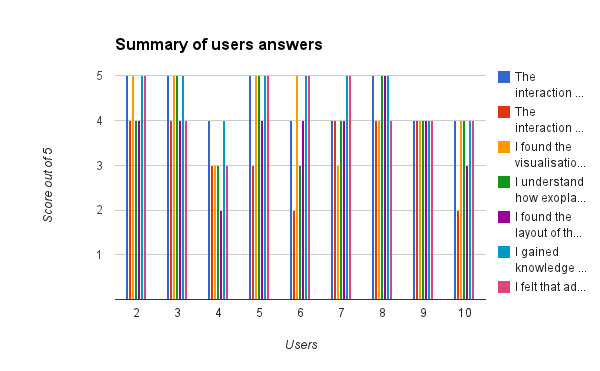
\includegraphics[width=0.8\textwidth]{images/charts/chart_9.png}
  \caption{Summary of results}  
    \label{fig:chart9}
    
\end{figure}
\section{Discussion}
Lack of control system.
Not evaluated in the evironment it is designed for ie observatory.
Not enough instruction 
Not all participants were comfortable moving around in 3d space
Some users had more trouble learning how to use the system than others
Users taking less time to become comfortable may not have experimented enough
with the visualisation

\section{Supporting Tools for project}
%Other tools used to support me
By supporting this project methodology with other project management tools such
as Gantt charts [APPENDIX~] and work breakdown structures(WBS) [APPENDIX~], it
encouraged efficient documentation of planning and work completed in the project
as well as displaying the upcoming stages required to complete the project.
\\

%Version Control
Version control was important for this project as it mitigated against the risks
of file system crashes and corruption, it also maintained effective revision
history that could be used to backtrack to or view changes that were made
earlier in the project. Version control was also valuable as it allowed me to
maintain multiple branches (versions) of my project that I could swap between.
This was important for the creation of the Keyboard and mouse system and the
Microsoft Kinect system as they were on separate branches in a repository. 

The version control tool that was used for this project was Git which allowed
for the repository to be hosted on the repository hosting web service Github.
This version control option was chosen due to the ease of use of as well as my
prior experience with Git which has all been positive. There was a minor
limitation of this choice as I used a free Github license which meant that the
repository would be open to the public.
\\

%Meetings with supervisor
Weekly meetings with the supervisor of the project, Dr Stuart Marshall, were
used to provide guidance and ideas for innovation of the visualisation
throughout the project. These meeting ensured that vital components and
deliverables were implemented in the required timeframe and also provided a
sounding board for ideas for elements to be included in the visualization.
Another important aspect of having an involved supervisor was that he provided
me the guidance of an experienced academic which was indispensable when
navigating the administrative side of organizing delicate matters such as ethics
approval for human evaluation of the visualisation.
